\documentclass[tikz,border=6pt]{standalone}
\usetikzlibrary{arrows.meta,calc}
\definecolor{red}{HTML}{A50F2D}\definecolor{ink}{HTML}{141414}\definecolor{gry}{HTML}{5F5F5F}
\newcommand{\wave}[3]{% x-offset, shift param, colour
 \draw[#3,very thick,smooth,samples=80,domain=0:3.4,xshift=#1 cm] plot (\x,{1.0+0.55*sin(deg(\x*2.2+#2))+0.25*sin(deg(\x*4.9+2*#2))});}
\begin{document}
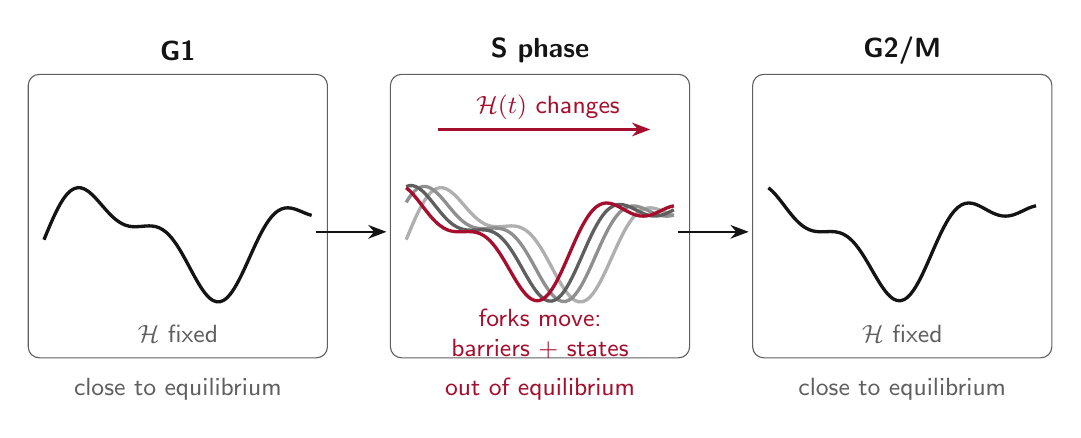
\begin{tikzpicture}[font=\sffamily\fontsize{11}{13}\selectfont,>=Stealth]
% panels
\foreach \x/\t in {0/{G1},4.6/{S phase},9.2/{G2/M}}{
  \draw[gry,rounded corners] (\x-0.2,-0.5) rectangle (\x+3.6,3.1);
  \node[ink,font=\sffamily\bfseries] at (\x+1.7,3.4) {\t};}
% G1: fixed landscape
\wave{0}{0}{ink}
\node[gry,font=\sffamily\small,align=center] at (1.7,-0.2) {$\mathcal{H}$ fixed};
% G2/M: fixed landscape
\wave{9.2}{1.3}{ink}
\node[gry,font=\sffamily\small,align=center] at (10.9,-0.2) {$\mathcal{H}$ fixed};
% S: landscape changes with time
\wave{4.6}{0}{gry!50}\wave{4.6}{0.5}{gry!70}\wave{4.6}{0.9}{gry}\wave{4.6}{1.3}{red}
\draw[->,red,thick] (5.0,2.4)--(7.7,2.4);
\node[red,font=\sffamily\small,anchor=south] at (6.4,2.4) {$\mathcal{H}(t)$ changes};
\node[red,font=\sffamily\small,align=center] at (6.3,-0.2) {forks move:\\barriers + states};
% arrows between panels
\draw[->,ink,thick] (3.45,1.1)--(4.35,1.1);
\draw[->,ink,thick] (8.05,1.1)--(8.95,1.1);
\node[gry,font=\sffamily\small] at (1.7,-0.9) {close to equilibrium};
\node[red,font=\sffamily\small] at (6.3,-0.9) {out of equilibrium};
\node[gry,font=\sffamily\small] at (10.9,-0.9) {close to equilibrium};
\end{tikzpicture}
\end{document}
